\documentclass{article}
\usepackage{tikz}
\usetikzlibrary{shapes.geometric, arrows.meta}

\begin{document}

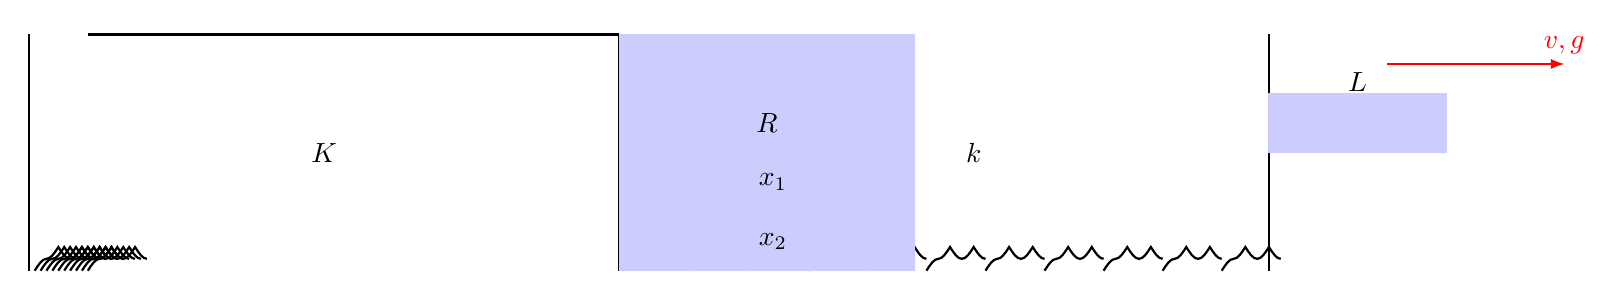
\begin{tikzpicture}[scale=0.75]
    % Draw the spring K
    \draw[thick] (0,0) -- (0,4);
    \foreach \x in {1,...,10} {
        \draw[thick] (\x/10,0) sin (\x/10+0.2,0.2) cos (\x/10+0.4,0.4)
            sin (\x/10+0.6,0.2) cos (\x/10+0.8,0.4) sin (\x/10+1,0.2);
    }
    \draw[thick] (10/10,4) -- (10,4);

    %标注弹簧K的参数
    \node at (5,2) {$K$};

    \draw[thick] (10,0) -- (10,4);
    
    % Draw the spring k
    \draw[thick] (11,0) -- (11,4);
    \foreach \x in {1,...,10} {
        \draw[thick] (\x+10.2,0) sin (\x+10.4,0.2) cos (\x+10.6,0.4)
            sin (\x+10.8,0.2) cos (\x+11,0.4) sin (\x+11.2,0.2);
    }
    \draw[thick] (21,4) -- (21,0);

    %标注弹簧k的参数
    \node at (16,2) {$k$};

    % Draw the masses
    \filldraw[blue!20] (10,0) rectangle (15,4) node[midway] {$M$};
    \filldraw[blue!20] (21,2) rectangle (24,3) node[midway] {$m$};

    %标注质量M和m的参数
    \node at (12.5,2.5) {$R$};
    \node at (12.6,1.5) {$x_1$};
    \node at (12.6,0.5) {$x_2$};
    \node at (22.5,3.2) {$L$};

    % Draw the velocity arrow
    \draw[-Latex, red] (23,3.5) -- (26,3.5) node[above] {$v, g$};

    %标注速度v和g的方向
\end{tikzpicture}

\end{document}